\documentclass{article}
\usepackage[catalan]{babel}
%\usepackage[latin1]{inputenc}   % Permet usar tots els accents i car鐃諸ers llatins de forma directa.
\usepackage[utf8]{inputenc}
\usepackage{enumerate}
\usepackage{amsfonts, amscd, amsmath, amssymb}
\usepackage[pdftex]{graphicx}
\usepackage{longtable}

\setlength{\textwidth}{16cm}
\setlength{\textheight}{24.5cm}
\setlength{\oddsidemargin}{-0.3cm}
\setlength{\evensidemargin}{0.25cm} \addtolength{\headheight}{\baselineskip}
\addtolength{\topmargin}{-3cm}

\newcommand\Z{\mathbb{Z}}
\newcommand\R{\mathbb{R}}
\newcommand\N{\mathbb{N}}
\newcommand\Q{\mathbb{Q}}
\newcommand\K{\Bbbk}
\newcommand\C{\mathbb{C}}

\newcounter{exctr}
\newenvironment{exemple}
{ \stepcounter{exctr} 
\hspace{0.2cm} 
\textit{Exemple  \arabic{exctr}: }
\it
\begin{quotation}
}{\end{quotation}}


\begin{document}

\textbf{\Large Tema 4.An\`alisi de Fourier i mostreig de senyals}

\vskip 0.2 cm
\textbf{\large An\`alisi de Fourier}

Per an\`alisi de Fourier ens referim a un conjunt de t\`ecniques matem\`atiques,
inspirades en els treballs de Joseph Fourier a principis del segle XIX, que
permeten descomposar qualsevol senyal en una suma de senyals sinuso\"idals
de diferents freq\"u\`encies.

Aquesta descomposici\'o \'es \'unica, de manera que es pot caracteritzar qualsevol 
senyal pel conjunt de freq\"u\`encies de les sinusoides que el composen. Per aquest
motiu l'an\`alisi de Fourier rep tamb\'e el nom d'\textbf{an\`alisi freq\"uencial}.

En funci\'o del tipus de senyal a analitzar les eines matem\`atiques per a l'an\`alisi
freq\"uencial varien i reben diferents noms (veure resum en la figura \ref{sumariFourier}):


\begin{description}

\item[Cas 1.] $x$ senyal anal\`ogic (temps continu) peri\`odic, de periode $T$:

\[
\begin{array}{ll}
x(t)=\displaystyle \sum_{k=-\infty}^{\infty} c_k e^{j \frac{2\pi k}{T} t} & \textbf{(s\`erie de Fourier)} \\ \\
c_k=\displaystyle \frac{1}{T} \int_T x(t) e^{-j \frac{2\pi k}{T} t} \, dt &
\end{array}
\]

\noindent
Propietats:
\begin{itemize}
\item An\`alisi freq\"uencial: freq\"u\`encies m\'ultiples de $\frac{1}{T}$.
\item La definici\'o de s\`erie de Fourier nom\'es t\'e sentit si el sumatori 
$\sum_{k=-\infty}^{\infty} c_k e^{j \frac{2\pi k}{T} t}$ convergeix per a tot valor de $t$.
En general, per a tots els senyals peri\`odics d'inter\'es es pot calcular la sèrie de Fourier.

\item Si $x(t)$ \'es un senyal real: 
\[
\displaystyle x(t)=c_0+ 2 \sum_{k=1}^\infty |c_k| \cos(\frac{2\pi k}{T} t + \theta_k)
\]
\noindent
on $c_k=|c_k|e^{j\theta_k}$. $|c_0|$ representa el valor mitj\`a del senyal en un periode.

\noindent
Si $x(t)$ \'es real i parell $x(-t)=x(t)$ llavors els coeficients $c_k$ s\'on reals. 
\noindent
Si $x(t)$ \'es real i imparell $x(-t)=-x(t)$ llavors els coeficients $c_k$ s\'on imaginaris purs. 

\item La pot\`encia del senyal $x$ es pot calcular a partir dels coeficients de la seva s\`erie de Fourier
(f\`ormula de Parseval).
(Recordem que l'energia dels senyals peri\`odics \'es infinita):
\[
P=\frac{1}{T} \int_T |x(t)|^2 \, dt = \sum_{k=-\infty}^\infty |c_k|^2
\]
\noindent
La representaci\'o dels valors de $|c_k|^2$ per a cada valor de freq\"u\`encia $\frac{k}{T}$ 
rep el nom d'\textbf{espectre de pot\`encia} o \textbf{densitat espectral de pot\`encia}.
Si el senyal \'es real llavors l'espectre de pot\`encia \'es sim\`etric respecte a l'eix vertical,
ja que $|c_{-k}| =|c_k|$. 


\end{itemize}

\vskip 0.2 cm
\noindent
\textbf{Exemple:} s\`erie de Fourier d'un pols rectangular peri\`odic

\begin{figure}[htbp]
\begin{center}
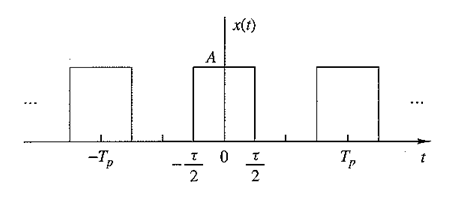
\includegraphics[width=6cm]{polsrectper.png} 
$\qquad$
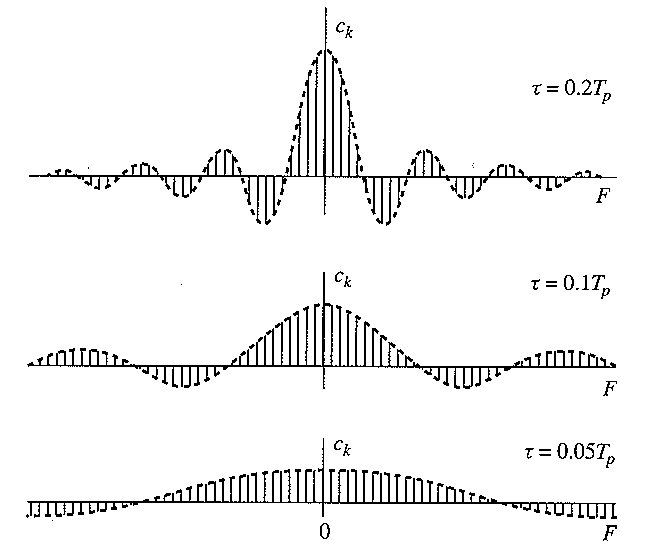
\includegraphics[width=6cm]{sincdiscret1.png} 
\end{center}
\caption{Senyal continu peri\`odic (pols rectangular d'amplada $\tau$) de periode $T_p$ i coeficients de la
seva s\`erie de Fourier per a diferents valors de $\tau$ amb $T_P$ fixat.}
\end{figure}

\newpage

\item[Cas 2.] $x$ senyal anal\`ogic (temps continu) no periòdic:

\[
\begin{array}{ll}
x(t)=\displaystyle \int_{-\infty}^{\infty} X(F) e^{j 2\pi F t} \, dF &  \\ \\
X(F)=\displaystyle \int_{-\infty}^{\infty} x(t) e^{-j 2\pi F t} \, dt & \textbf{(transformada de Fourier)}
\end{array}
\]

\noindent
Alternativament, aquestes expressions es poden escriure en termes de la freq\"u\`encia angular $\Omega=2\pi F$:

\[
\begin{array}{ll}
x(t)=\frac{1}{2\pi} \displaystyle \int_{-\infty}^{\infty} X(\Omega) e^{j \Omega t} \, d\Omega &  \\ \\
X(\Omega)=\displaystyle \int_{-\infty}^{\infty} x(t) e^{-j \Omega t} \, dt & \textbf{(transformada de Fourier)}
\end{array}
\]

\noindent $X(F)$ rep el nom d'\textbf{espectre del senyal} i tamb\'e es denota com ${\cal F}(x(t))$.
La transformada inversa de Fourier es denota ${\cal F}^{-1}(X(F))=x(t)$.

\noindent
Propietats:
\begin{itemize}
\item An\`alisi freq\"uencial: totes les freq\"u\`encies.

\item La definici\'o de transformada de Fourier nom\'es t\'e sentit si la integral 
$\int_{-\infty}^{\infty} x(t) e^{-j \Omega t} \, dt$ convergeix per a tot valor de $t$.
En la pr\`actica, per a tots els senyals que trobarem en el ``mon real'' podrem calcular
les seves transformades i transformades inverses de Fourier.
\item L'energia del senyal $x$ es pot calcular a partir dels coeficients de la seva transformada de Fourier
(f\`ormula de Parseval):
\[
E=\int_{-\infty}^\infty |x(t)|^2 \, dt = \int_{-\infty}^\infty |X(F)|^2 \, df
\]

S'anomena \textbf{densitat espectral d'energia} a la funci\'o $S_{XX}(F)=|X(F)|^2$.

\item si $x(t)$ \'es un senyal real llavors $|X(-F)|=|X(F)|$ (espectre sim\`etric respecte a l'eix vertical)
i $S_{XX}(-F)=S_{XX}(F)$.


\end{itemize}

\vskip 0.2 cm
\noindent
\textbf{Exemple:} transformada de Fourier d'un pols rectangular

\begin{figure}[htbp]
\begin{center}
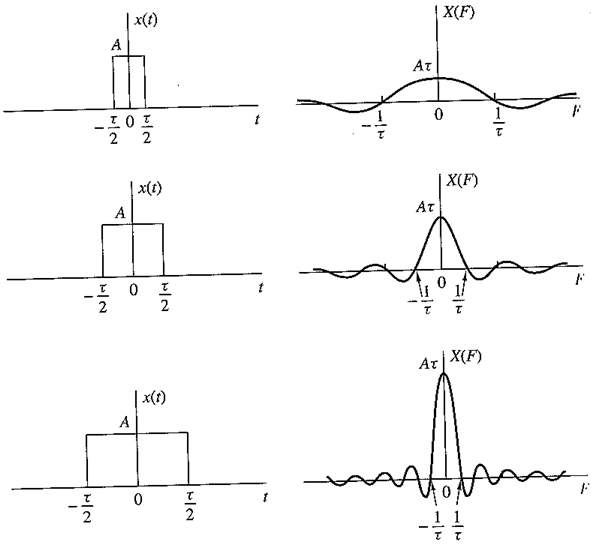
\includegraphics[width=8cm]{polsrectitransfF2.png} 
\end{center}
\caption{Senyal continu no peri\`odic (pols rectangular d'amplada $\tau$) i la
seva transformada de Fourier per a diferents valors de $\tau$.}
\end{figure}

\newpage
\item[Cas 3.] $x$ senyal digital (temps discret) peri\`odic de periode $N$:

\[
\begin{array}{ll}
x[n]=\displaystyle \sum_{k=0}^{N-1} c_k e^{j \frac{2\pi k}{N} n} \qquad n=0, \cdots, N-1&  \textbf{(s\`erie discreta de Fourier)}\\ \\
c_k=X[k]=\displaystyle \frac{1}{N} \sum_{n=0}^{N-1} x[n] e^{-j \frac{2\pi k}{N} n} \qquad k=0, \cdots, N-1 & 
\textbf{(transformada discreta de Fourier (DFT))}
\end{array}
\]

\noindent
Propietats
\begin{itemize}
\item An\`alisi freq\"uencial: $N$ freq\"u\`encies m\'ultiples de $\frac{1}{N}$ (de $f=0$ fins a $f=\frac{N-1}{N}$).
\item La s\`erie discreta de Fourier sempre es pot calcular.
\item Els coeficients $c_k$ formen una seq\"u\`encia peri\`odica de periode $N$, ja que $c_k=c_{k+N}$.
\item La representaci\'o dels coeficients $c_k$ per a cada valor de $k$ rep el nom d'\textbf{espectre} del senyal.
\item La pot\`encia del senyal $x$ es pot calcular a partir dels coeficients de la seva s\`erie de Fourier
(f\`ormula de Parseval):
\[
P=\frac{1}{N} \sum_{k=0}^{N-1} |x[n]|^2  = \sum_{k=0}^{N-1} |c_k|^2
\]
\noindent
La representaci\'o dels valors de $|c_k|^2$ per a cada valor de freq\"u\`encia $\frac{k}{N}$ 
rep el nom d'\textbf{espectre de pot\`encia} o \textbf{densitat espectral de pot\`encia}.
Si el senyal \'es real llavors l'espectre de pot\`encia \'es sim\`etric respecte a l'eix vertical,
ja que $|c_{-k}| =|c_k|$. 
\end{itemize}

\vskip 0.2 cm
\noindent
\textbf{Exemple:} s\`erie de Fourier d'un pols rectangular discret peri\`odic

\begin{figure}[htbp]
\begin{center}
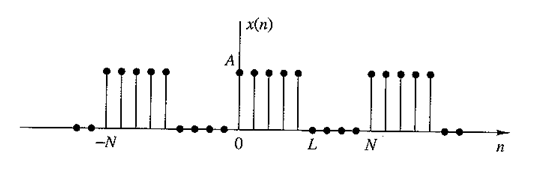
\includegraphics[width=6cm]{polsrectperdiscret.png} 
$\qquad$
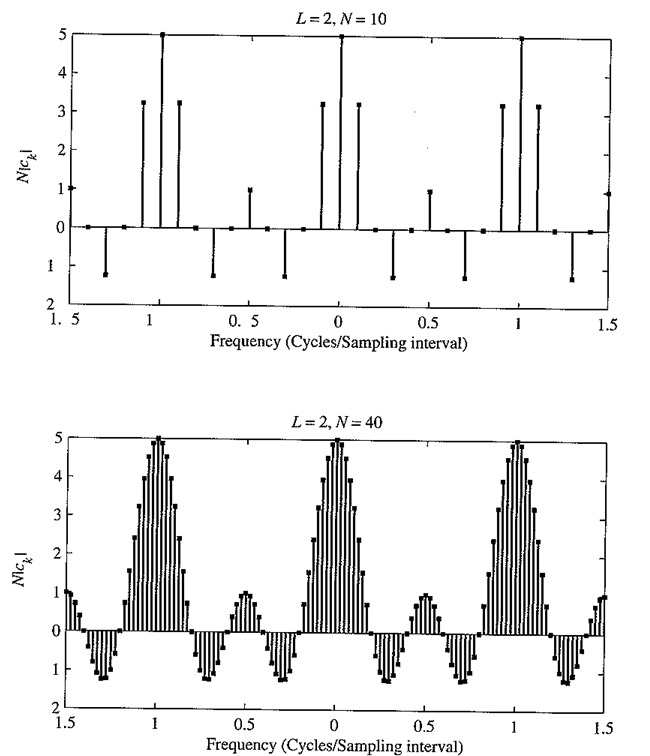
\includegraphics[width=6cm]{sincdiscret.png} 
\end{center}
\caption{Senyal discret peri\`odic (pols rectangular d'amplada $L$) de periode $N$ i coeficients de la
seva s\`erie de Fourier (transformada de Fourier discreta) per a diferents valors de $N$ amb $L$ fixat.
Notem que la transformada discreta \'es tamb\'e peri\`odica amb periode $N$. En la figura de la dreta
l'eix horitzontal representa els valors de freq\"u\`encia $f=k/N$.}
\end{figure}


\item[Cas 4.] $x$ senyal digital (temps discret) no peri\`odic:

\[
\begin{array}{ll}
x[n]=\displaystyle \int_0^1 X(f) e^{j 2 \pi f n} \, df & \\ \\
X(f)=\displaystyle \sum_{n=-\infty}^\infty x[n] e^{-j 2 \pi f n} & \textbf{Transformada de Fourier en temps discret}
\end{array}
\]

\noindent
Alternativament, aquestes expressions es poden escriure en termes de la freq\"u\`encia angular $\omega=2\pi f$:

\[
\begin{array}{ll}
x[n]=\displaystyle \frac{1}{2\pi} \int_0^{2\pi} X(\omega) e^{j \omega n} \, d\omega & \\ \\
X(\omega)=\displaystyle \sum_{n=-\infty}^\infty x[n] e^{-j \omega n} & \textbf{Transformada de Fourier en temps discret}
\end{array}
\]

\noindent
Propietats
\begin{itemize}
\item An\`alisi freq\"uencial: totes les freq\"u\`encies entre $0$ i $1$ (o, de manera equivalent, $\omega \in (0, 2\pi)$).
\item $X(\omega)$ \'es peri\`odica amb periode $2\pi$: $X(\omega+2\pi k)=X(\omega)$, per a tot $k$
\item La transformada de Fourier en temps discret existeix si $x(t)$ \'es absolutament sumable ($\sum_n |x[n]| < \infty$)
o b\'e si \'es d'energia finita ($\sum_n |x[n]|^2 < \infty$).
\item L'energia del senyal $x$ es pot calcular a partir dels coeficients de la seva transformada de Fourier en temps discret
(f\`ormula de Parseval):
\[
E=\sum_{n=-\infty}^\infty |x[n]|^2 = \frac{1}{2\pi} \int_{-\pi}^\pi |X(\omega)|^2 \, d\omega
\]

S'anomena \textbf{densitat espectral d'energia} a la funci\'o $S_{XX}(\omega)=|X(\omega)|^2$.

\item si $x[n]$ \'es un senyal real llavors $|X(-\omega)|=|X(\omega)|$ (espectre sim\`etric respecte a l'eix vertical)
i $S_{XX}(-\omega)=S_{XX}(\omega)$.

\end{itemize}

\vskip 0.2 cm
\noindent
\textbf{Exemple:} transformada de Fourier d'un pols rectangular discret no peri\`odic

\begin{figure}[htbp]
\begin{center}
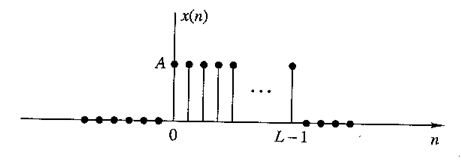
\includegraphics[width=6cm]{polsrectdiscret.png} 
$\qquad$
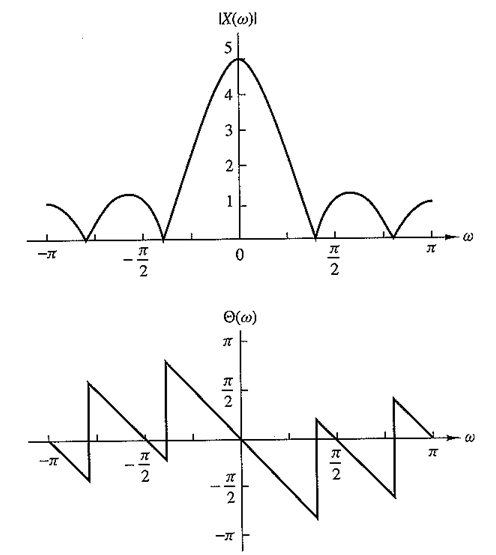
\includegraphics[width=6cm]{polsrectdiscretTF.png} 
\end{center}
\caption{Senyal discret no peri\`odic (pols rectangular d'amplada $L$) i la
seva transformada de Fourier (m\`odul i fase).
Notem que la transformada de Fourier $X(\omega)$ \'es peri\`odica amb periode $2\pi$.}
\end{figure}



\newpage
\noindent
\textbf{Relaci\'o entre la transformada de Fourier en temps discret i la transformada Z}

\noindent
Comparant les definicions de la transformada Z i la transformada de Fourier d'un senyal discret
podem trobar la seg\"uent relaci\'o:

\[
X(\omega)=X(z)|_{z=e^{j\omega}}=\sum_{n=-\infty}^\infty x[n] e^{-j\omega n}
\]

\noindent
Per a que aquesta relaci\'o sigui certa s'han de cumplir que
la transformada Z estigui definida per a $z=e^{j\omega}$, \'es a dir $z=e^{j\omega}$ ha de pert\`anyer a la ROC
de $X(z)$, la qual cosa equival a dir que la ROC de $X(z)$ cont\'e el cercle unitat.

\vskip 0.3 cm
\noindent
\textbf{Propietats de simetria de la transformada de Fourier en temps discret}

\begin{center}
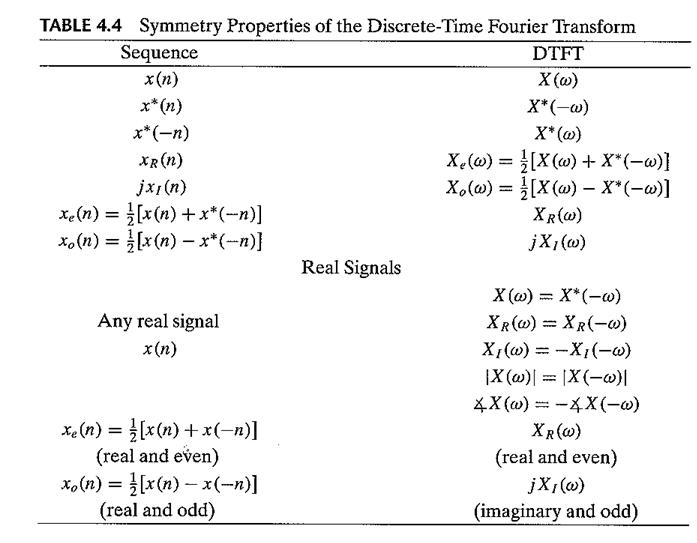
\includegraphics[width=10cm]{tabpropsimetria.png}
\end{center}


\newpage
\noindent
\textbf{Altres propietats de la transformada de Fourier en temps discret}

\begin{center}
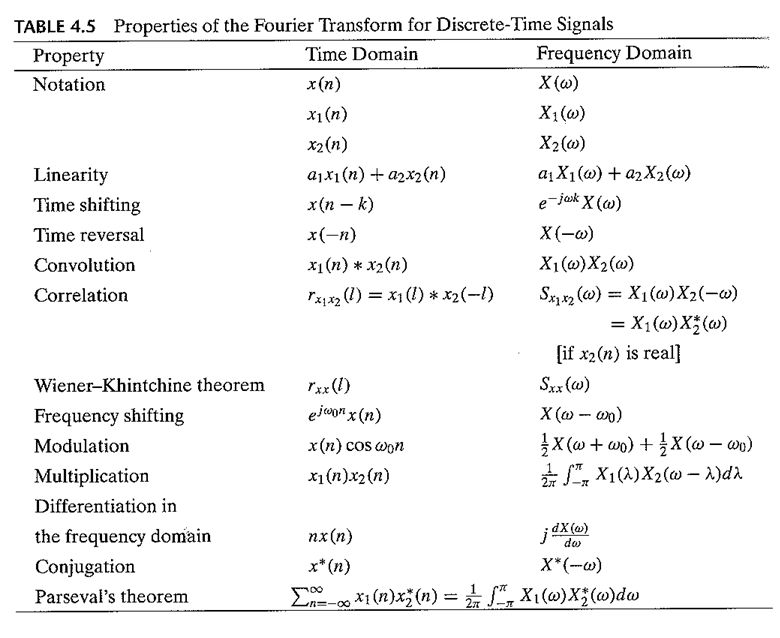
\includegraphics[width=10cm]{tabpropTF.png}
\end{center}

\vskip 0.3 cm
\noindent
\textbf{Parells transformats habituals per a senyals discrets aperi\`odics} 

\begin{center}
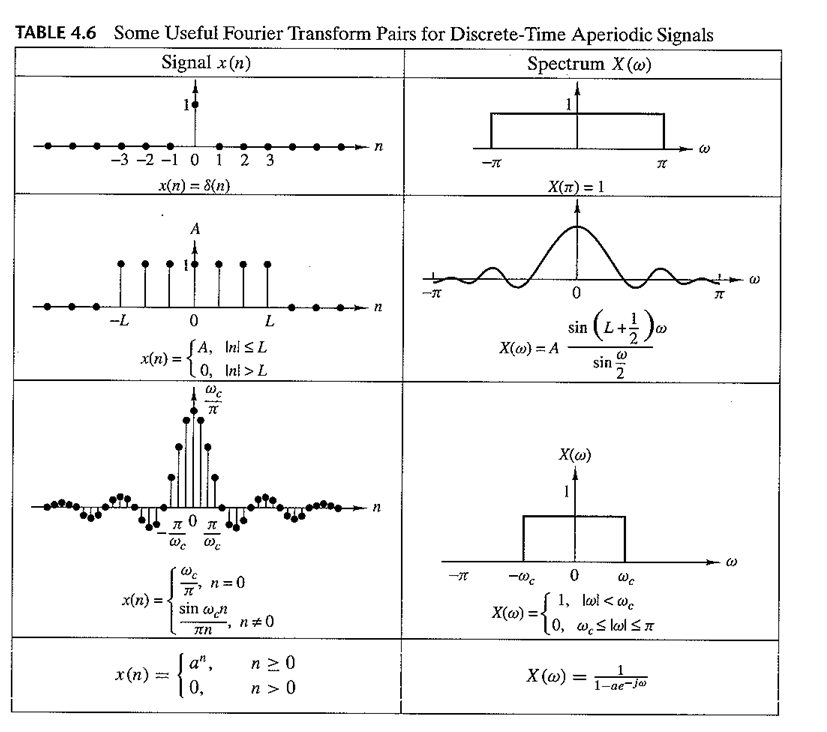
\includegraphics[width=10cm]{tabTFpairs.png}
\end{center}


\end{description}



\begin{figure}[htbp]
\begin{center}
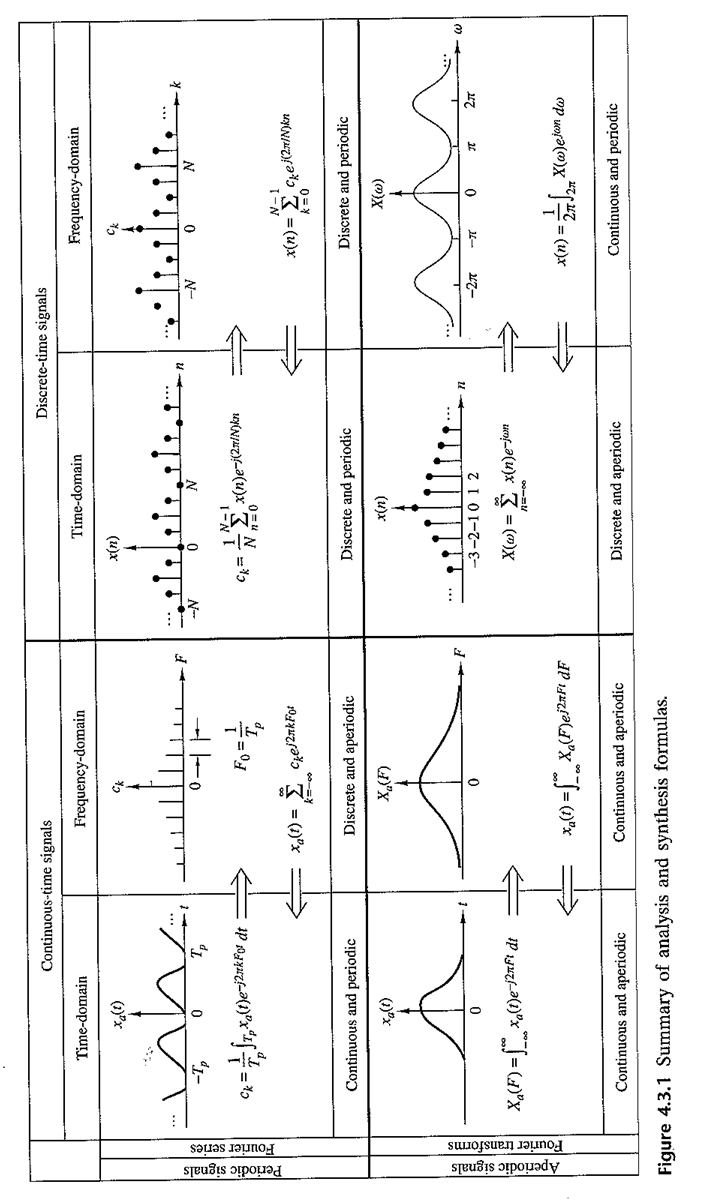
\includegraphics[height=20cm]{sumariTF.png}
\end{center}
\caption{Font: Digital Signal Processing, J. Proakis, D. Manolakis, Pearson Prentice Hall, 2007}
\label{sumariFourier}
\end{figure}




\noindent
\textbf{Relaci\'o entre la Transformada Discreta de Fourier i la Transformada de Fourier en temps discret}

Consideram un senyal discret finit $x[n]$ que pren valors entre $n=0$ i $n=N-1$.
Com es tracta d'un senyal no peri\`odic podem calcular la seva Transformada de Fourier en temps discret:

\[
X(\omega)=\sum_{n=-\infty}^\infty x[n] e^{-j\omega n}=\sum_{n=0}^{N-1} x[n] e^{-j\omega n}
\]

D'altra banda podem considerar l'extensi\'o peri\`odica d'aquest senyal:
\[
x_P[n]=x[n] \qquad \text{si } n=0, \cdots, N-1 \qquad \qquad x_P[n+N]=x_P[n] \quad \text{per a tot } n
\]
\noindent
Observem que per a valors de $n$ entre $0$ i $N-1$ ambd\'os senyals s\'on id\`entics.

\vskip 0.3 cm
\noindent
Aquest nou senyal \'es peri\`odic i per tant podem calcular la seva Transformada Discreta de Fourier:
\[
X_P[k]=\frac{1}{N}\sum_{n=0}^{N-1} x_P[n] e^{-j \frac{2 \pi k}{N} n} =\frac{1}{N}\sum_{n=0}^{N-1} x[n] e^{-j \frac{2 \pi k}{N} n} 
\]

\vskip 0.3 cm
\noindent
Ens demanam per la relaci\'o entre aquestes dues transformades. Comparant les expressions obtingudes observam que:
 
\[
X_P[k]=\frac{1}{N}X(\frac{2\pi k}{N})
\]

\'es a dir, la DFT \'es una versi\'o discreta i reescalada de la Transformada de Fourier del senyal discret.


\vskip 0.3 cm
La conclusi\'o del raonament anterior \'es que \'es possible con\`eixer, de manera aproximada, 
la transformada de Fourier d'un senyal discret a partir de la DFT de la seva versi\'o perioditzada.
En la pr\`actica \'es molt m\'es f\`acil calcular la DFT que la transformada de Fourier, ja que existeixen
algoritmes r\`apids de c\`alcul (anomenats FFT: \textit{Fast Fourier Transform}), amb la ventatja
que el resultat \'es un senyal discret que pot \'esser enmagatzemat en l'ordinador. Per aquest motiu
normalment es calcula la DFT i a partir d'ella es dedueixen propietats de la Transformada de Fourier del senyal.


\vskip 0.4 cm
\noindent
\textbf{Exemple:} comparaci\'o de la transformada de Fourier de $x[n]=a^n u[n]$ (amb $a=0.8$) i la seva transformada
discreta de Fourier (figures \ref{exTFDFT1} i \ref{exTFDFT2}).

\begin{figure}[htbp]
\begin{center}
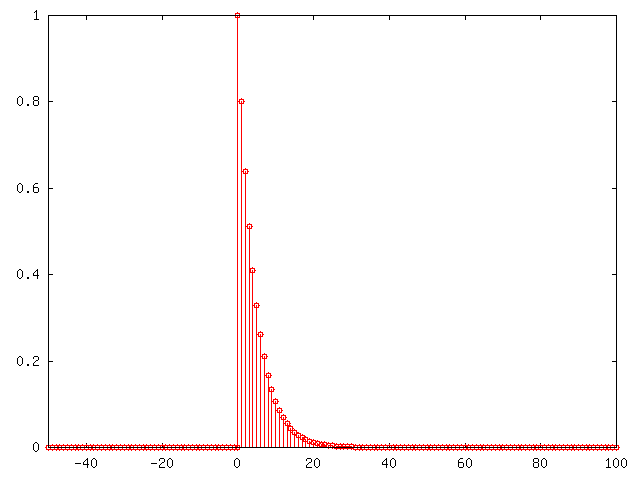
\includegraphics[width=6cm]{signal0_T4.png} 
$\qquad$
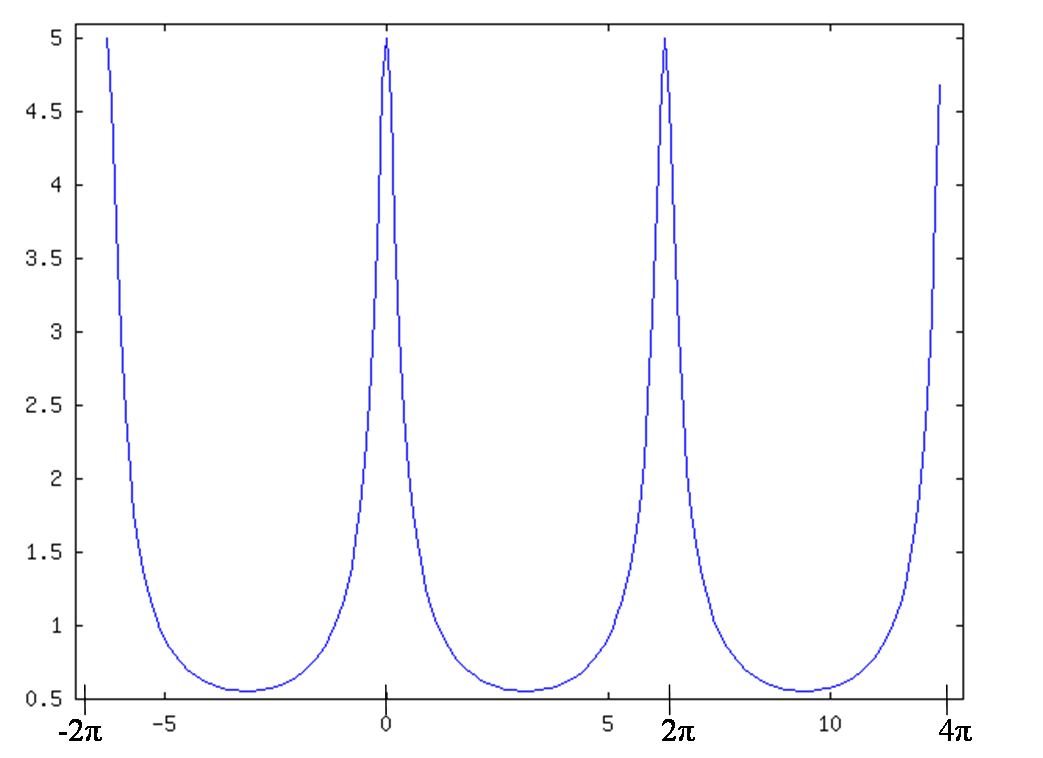
\includegraphics[width=6cm]{TFsignal0bis_T4.png} 
\end{center}
\caption{Senyal discret no peri\`odic i la seva transformada de Fourier .
Notem que la transformada de Fourier $X(\omega)$ \'es peri\`odica amb periode $2\pi$.}
\label{exTFDFT1}
\end{figure}

\begin{figure}[htbp]
\begin{center}
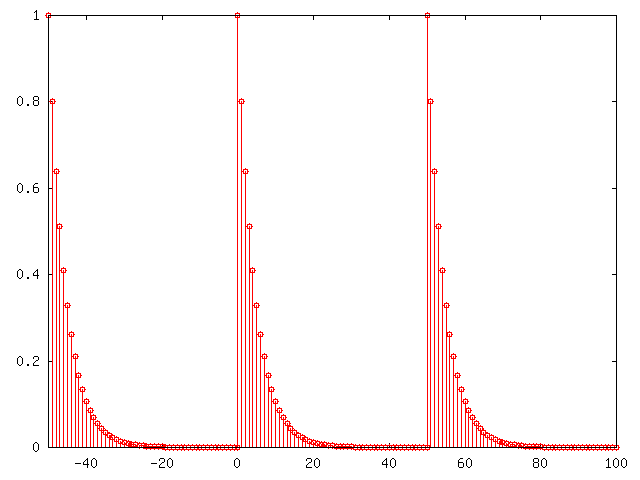
\includegraphics[width=6cm]{signal0P_T4.png} 
$\qquad$
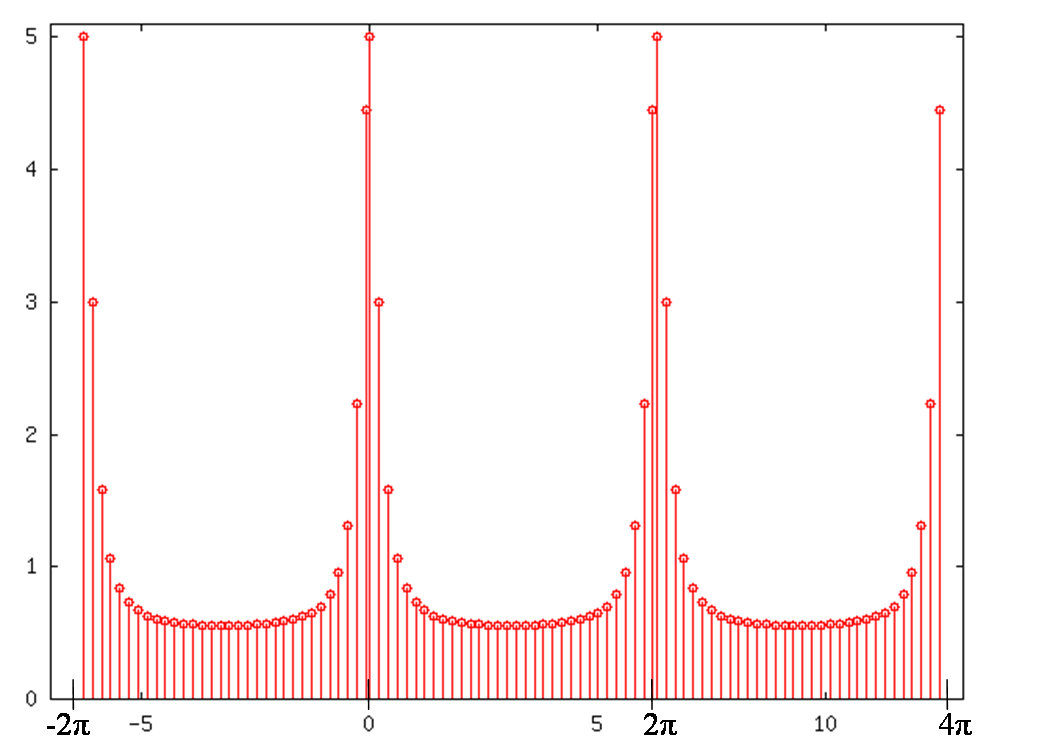
\includegraphics[width=6cm]{TFsignal0Pbis_T4.png} 
\end{center}
\caption{Senyal discret perioditzat (periode $N=50$) i coeficients de la seva s\`erie de Fourier (transformada discreta de Fourier).
Notem que la DFT \'es un versi\'o discreta de la transformada de Fourier del senyal no peri\`odic. La dist\`ancia
entre les mostres \'es $\frac{2\pi}{N}$.}
\label{exTFDFT2}
\end{figure}




\newpage
\textbf{\large Mostreig de senyals}

En aquesta secci\'o estudiam el proc\'es de mostreig de senyals. L'objectiu del mostreig
\'es representar amb un nombre discret de valors (\textit{mostres}) un senyal anal\`ogic (temps continu)
o b\'e representar amb un nombre menor de mostres un senyal digital (temps discret).
Estudiarem el proc\'es de mostreig tant des del punt de vista temporal com des del punt de vista freq\"uencial
i establirem quines condicions ha de verificar el proc\'es per fer possible la recuperaci\'o del senyal
mostrejat original a partir de les seves mostres.


\vskip 0.3 cm
\noindent
\textbf{Mostreig de senyals anal\`ogics}

La figura \ref{figmostreig} il.lustra el proc\'es de mostreig d'un senyal anal\`ogic. El senyal discret obtingut
$x[n]$ \'es igual al senyal original $x_a(t)$ per als valors de $t=nT$, on $T$ rep el nom de \textbf{periode de
mostreig}: $x[n]=x_a(nT)$.

\begin{figure}[htbp]
\begin{center}
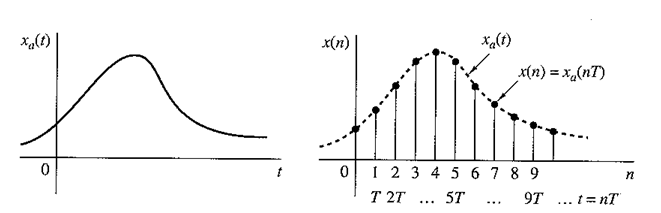
\includegraphics[width=8cm]{figmostreig.png}
\end{center}
\caption{Mostreig d'un senyal continu amb un periode de mostreig $T$.}
\label{figmostreig}
\end{figure}

\vskip 0.2 cm
\noindent
\textbf{Freq\"u\`encies de senyals continus i de senyals discrets}

Per a estudiar el proc\'es de mostreig des del punt de vista freq\"uencial calcularem les transformades de
Fourier de $x_a(t)$ i $x[n]$ aplicant les f\`ormules estudiades en les seccions anteriors (casos 2 i 4, respectivament),
per\`o cal tenir en compte que les ``freq\"u\`encies'' a les quals fan refer\`encia les f\`ormules representen
magnituds diferents en el cas continu i en el cas discret.

En el cas continu la freq\"u\`encia representa el \textit{nombre de cicles per segon} o \textit{hertz} (Hz) (veure la 
Figura \ref{figfreq}-esquerra).


En el cas continu la freq\"u\`encia representa el \textit{nombre de cicles per mostra} (veure la 
Figura \ref{figfreq}-dreta).


\begin{figure}[htbp]
\begin{center}
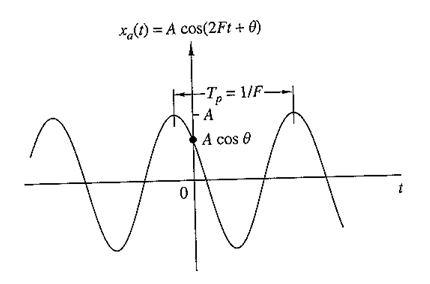
\includegraphics[width=6cm]{ciclessegon.png}
$\qquad$
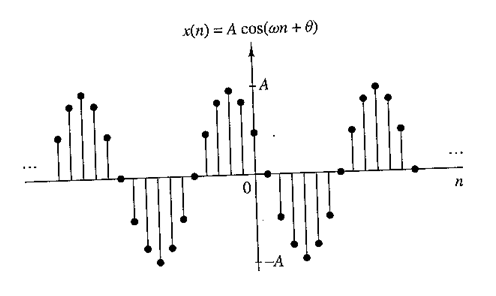
\includegraphics[width=6cm]{ciclesmostra.png}
\end{center}
\caption{Difer\`encia entre la freq\"u\`encia d'un senyal continu (esquerra) i la d'un senyal discret (dreta).}
\label{figfreq}
\end{figure}


Per distingir ambdues magnituds utilitzarem la lletra $F$ per denotar la freq\"u\`encia 
d'un senyal continu i $f$ per denotar la d'un senyal discret
(tamb\'e utilitzarem la notaci\'o $\Omega$ i $\omega$ per distingir entre freq\"u\`encia angular
dels senyals continus i dels senyals discrets, respectivament).
La relaci\'o entre ambues freq\"u\`encies \'es $F=\frac{f}{T}$ (resp., $\Omega=\frac{\omega}{T}$).


\vskip 0.2 cm
\noindent
\textbf{Relaci\'o entre els espectres de $x_a(t)$ i $x[n]$}
La relaci\'o entre les transformades $X_a$ i $X$ v\'e donada per la seg\"uent expressi\'o:

\[
X(f)=X(FT)=\frac{1}{T} \sum_{k=-\infty}^\infty X_a(F+\frac{k}{T})
\]

\noindent
o de manera equivalent, en termes de $\Omega$ i $\omega$:

\[
X(\omega)=X(\Omega T)=\frac{1}{T} \sum_{k=-\infty}^\infty X_a(\Omega+2\pi\frac{k}{T})
\]

\noindent
\'Es a dir, la transformada del senyal discret s'obt\'e com la superposici\'o de transformades del senyal
continu despla\c{c}ades en freq\"u\`encia a intervals regulars $\frac{1}{T}$.
La figura \ref{exmostreig} il.lustra l'efecte del mostreig en l'espectre d'un senyal.

\vskip 0.2cm
\noindent
La relaci\'o entre $X_a$ i $X$ es pot deduir a partir de les f\`ormules de les transformades descrites en les
seccions anteriors (casos 2 i 4, respectivament). Alternativament, es pot obtenir la relaci\'o entre
aquestes transformades fent us de la versi\'o continua $\hat{x}(t)$ del senyal discret $x[n]=x_a(nT)$, que es
defineix com:
\[
\hat{x}(t)=x_a(t) \cdot \sum_{n=-\infty}^\infty \delta(t-nT)
\]

\noindent
on el sumatori $\sum_{n=-\infty}^\infty \delta(t-nT)$ rep del nom de \textbf{tren de deltes}. $\delta(t)$
es defineix de manera que $\int_{-\infty}^\infty f(t) \delta(t-t_0) \, dt = f(t_0)$ per a qualsevol funci\'o $f(t)$.
Amb aquesta definici\'o es verifica que $\hat{X}(F)=X(FT)$. A m\'es es pot comprovar que $\hat{X}(F)=\frac{1}{T} \sum_{k=-\infty}^\infty X_a(F+\frac{k}{T})$.

\begin{figure}[htbp]
\begin{center}
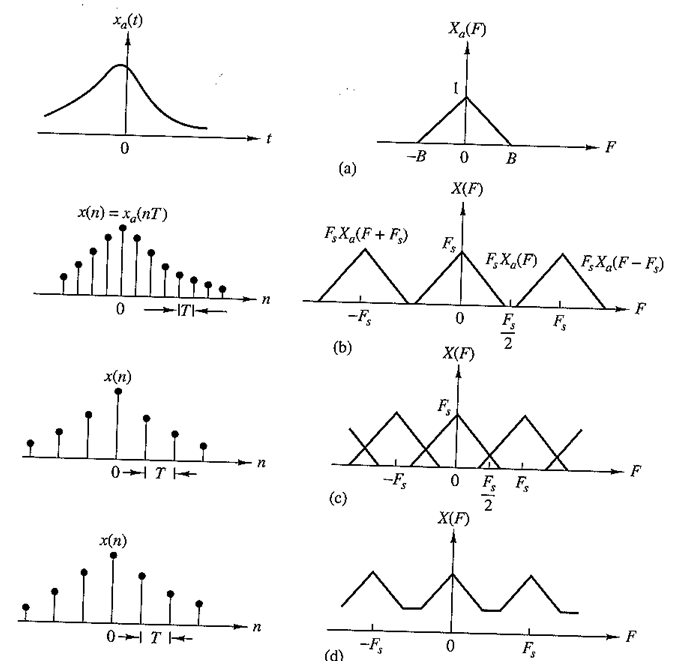
\includegraphics[height=8cm]{exmostreig.png}
\end{center}
\caption{(a) Senyal original i el seu espectre. Notem que el senyal t\'e amplada de banda limitada i que l'espectre
s'anul.la quan $|F|>B$. (b) Senyal mostrejat amb un periode de mostreig $T$ tal que $T < \frac{1}{2B}$ i el seu espectre.
(c) Senyal mostrejat amb un periode de mostreig $T$ tal que $T > \frac{1}{2B}$ i proc\'es de formaci\'o del seu espectre.
(d) Senyal mostrejat amb un periode de mostreig $T$ tal que $T > \frac{1}{2B}$ i el seu espectre.}
\label{exmostreig}
\end{figure}

\vskip 0.3 cm
\noindent
\textbf{Teorema del mostreig (teorema de Shannon-Whitaker)}

Ens demanam en aquesta secci\'o si \'es possible recuperar el senyal continu original a partir de la 
seva versi\'o mostrejada. La resposta \'es s\'i, sempre que la relaci\'o entre l'amplada de banda del
senyal original i la freq\"u\`encia de mostreig sigui l'adequada.
Observant la figura \ref{exmostreig} podem deduir quina \'es aquesta condici\'o:
\renewcommand{\labelitemi}{-}
\begin{itemize}
\item Si $T$ \'es massa gros (\'es a dir, la freq\"u\`encia de mostreig $F_m=\frac{1}{T}$ 
\'es massa petita) les repeticions de l'espectre original es solapen (aquest fen\`omen
rep el nom d'\textbf{aliasing}) (veure (c))
i \'es impossible identificar l'espectre original en l'espectre resultant (veure (d)).
\item En canvi, si $T$ \'es suficientment petit (\'es a dir, $F_m$ \'es suficientment gros), llavors
s\'i es possible identificar l'espectre original en l'espectre resultant (veure (b)).
\end{itemize}

La condici\'o que ha de cumplir la freq\"u\`encia de mostreig per a poder recuperar el senyal original
a partir del mostrejat s'anomena \textbf{condici\'o de Nyquist}, i la freq\"u\`encia m\'inima
de mostreig rep el nom de \textbf{freq\"u\`encia de Nyquist} ($F_N$):
\[
F_m > 2B \qquad \text{per tant} \qquad F_N=2B
\]

En cas que un senyal hagi estat mostrejat satisfent la condici\'o de Nyquist, el \textbf{teorema del
mostreig} ens diu com obtenir el senyal original a partir del mostrejat: 
\begin{itemize}
\item Definim $X_{\Pi}(F)=X(FT) \cdot H_{\Pi}(F)$, on
$H_{\Pi}(F)=\begin{cases} T & \text{ si } |F| \leq F_m/2 \\ 0 & \text{altrament} \end{cases}=
\begin{cases} T & \text{ si } |F| \leq 1/2T \\ 0 & \text{altrament} \end{cases}$
\item Si es verifica la condici\'o de Nyquist llavors $X_{\Pi}(F)=X_a(F)$ 
\item Calculam $x_a(t)$ com la transformada inversa de $X_{\Pi}(F)$:
\[
x_a(t)=\int_{-\infty}^\infty X_{\Pi}(F) e^{j 2 \pi F t} \, dF
\]
\item El resultat del c\`alcul d\'ona:
\[
x_a(t)=\sum_{n=-\infty}^\infty x[n] \frac{\sin(\frac{\pi(t-nT)}{T})}{\frac{\pi(t-nT)}{T}}=
\sum_{n=-\infty}^\infty x[n] \cdot \mathrm{sinc}(\frac{\pi(t-nT)}{T})
\]
\noindent
on $\mathrm{sinc}(x)=\frac{\sin x}{x}$.
\end{itemize}

El proc\'es de reconstrucci\'o del senyal original a partir de les seves mostres s'il.lustra 
a les figures \ref{exrecons1} i \ref{exrecons2}. En cas que el senyal mostrejat no satisfaci les condicions de Nyquist
el senyal reconstru\"it \'es diferent de l'original (figura \ref{exmalarecons}).

\begin{figure}[htbp]
\begin{center}
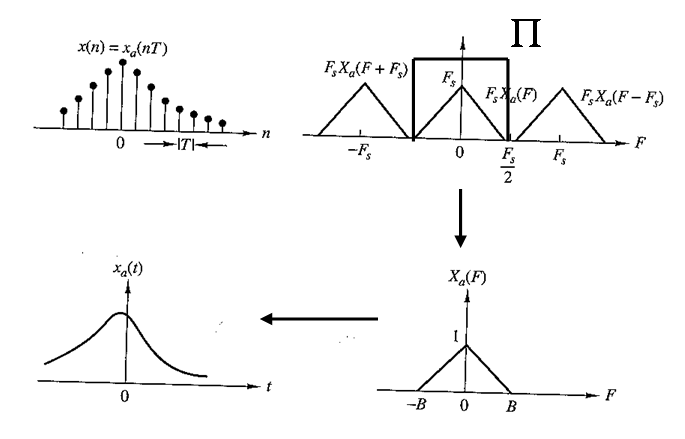
\includegraphics[width=8cm]{exrecons1.png}
\end{center}
\caption{Reconstrucci\'o del senyal anal\`ogic a partir d'un senyal digital mostrejat correctament}
\label{exrecons1}
\end{figure}

\begin{figure}[htbp]
\begin{center}
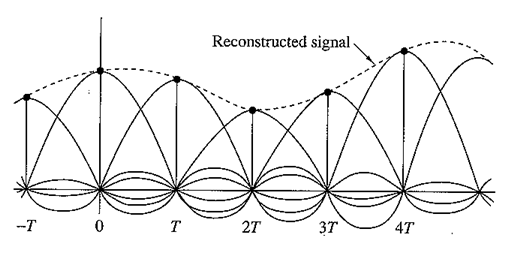
\includegraphics[width=6cm]{exrecons2.png}
\end{center}
\caption{Il.lustraci\'o del proc\'es de reconstrucci\'o del senyal anal\`ogic a partir de les
seves mostres utilitzant la f\`ormula del teorema del mostreig.}
\label{exrecons2}
\end{figure}

\begin{figure}[htbp]
\begin{center}
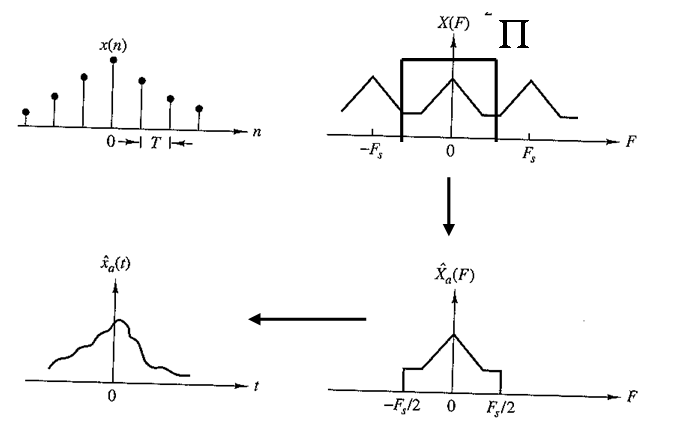
\includegraphics[width=8cm]{exmalarecons.png}
\end{center}
\caption{Dalt, senyal mostrejat sense cumplir la condici\'o de Nyquist i el seu espectre.
Baix, a la dreta, $X_{\Pi}(F)$ corresponent al senyal anterior. Esquerra, reconstrucci\'o del
senyal a partir de $X_{\Pi}(F)$. Comparau amb la figura \ref{exrecons1}.}
\label{exmalarecons}
\end{figure}


\vskip 0.3 cm
\noindent
\textbf{Mostreig de senyals discrets (delmat)}

Volem estudiar el senyal $x_M[n]=x[Mn]$, on $M$ \'es un enter positiu (veure exemple a la figura \ref{exmostreigdiscret}).
El resultat del mostreig \'es un nou senyal discret equivalent a mostrejar el senyal anal\`ogic
original amb un periode de mostreig $MT$ ($T$ \'es el periode de mostreig original).
A nivell freq\"uencial, es pot calcular l'espectre de $x_M[n]$ a partir del de $x[n]$:
\[
X_M(f)=\frac{1}{M} \sum_{k=0}^{M-1} X(\frac{f}{M}-\frac{k}{M})
\]
Observam que el resultat del mostreig \'es un apropament de les repeticions de l'espectre del senyal
anal\`ogic original. Si $M$ \'es massa gros s'arriba a produir aliasing.

\begin{figure}[htbp]
\begin{center}
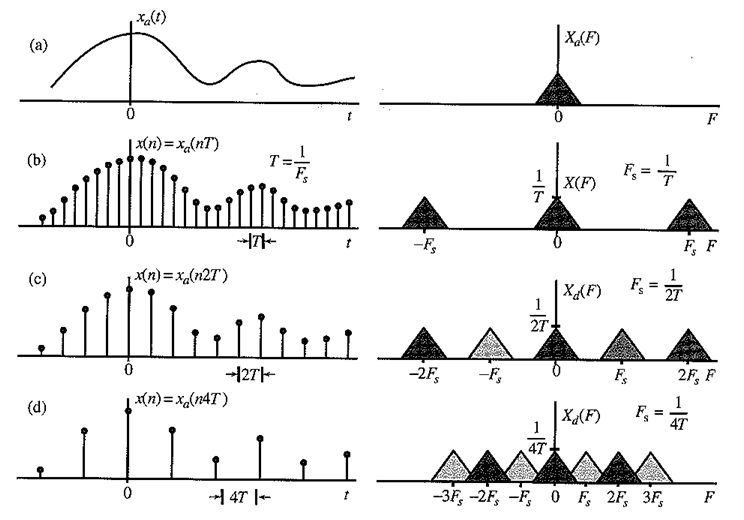
\includegraphics[width=8cm]{exmostreigdiscret.png}
\end{center}
\caption{Exemples de delmat d'un senyal discret}
\label{exmostreigdiscret}
\end{figure}


\vskip 0.5 cm
\noindent
\textbf{\large Processament digital de senyals anal\`ogics}

Considerem un senyal anal\`ogic $x_a(t)$ que es processa amb un sistema ${\cal T}_a$ per donar
com a sortida el senyal $y_a(t)$.

\begin{center}
\begin{minipage}{6cm} 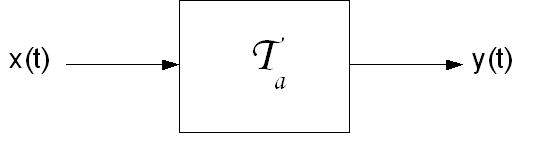
\includegraphics[width=6cm]{sistemaanalogic.png}\end{minipage}
\end{center}

Considerem ara la versi\'o discreta del senyal: $x[n]=x_a(nT)$.

\noindent
\textbf{Propietat:} 

\noindent
Si ${\cal T}_a$ \'es un sistema LTI i 
$T$ \'es un periode de mostreig que satisf\`a la condici\'o de Nyquist llavors es pot trobar
un sistema digital ${\cal T}$ LTI amb funci\'o de transfer\`encia $H(f)$ tal que la
seva sortida $y[n]$ \'es la versi\'o discreta del senyal $y_a(t)$. Es diu en aquest cas
que els sistemes ${\cal T}_a$ i ${\cal T}$ s\'on equivalents.

\vskip 0.3 cm
\noindent
La relaci\'o entre ${\cal T}_a$ i ${\cal T}$ es pot representar amb el seg\"uent diagrama de blocs:

\begin{center}
\begin{minipage}{10cm} 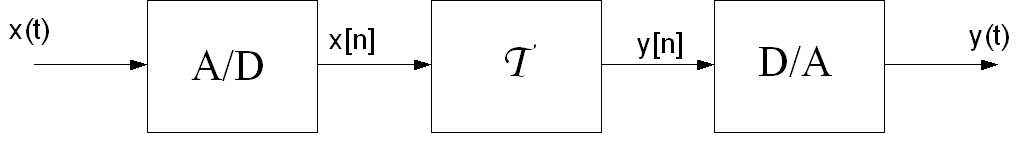
\includegraphics[width=10cm]{sistemadigital.png}\end{minipage}
\end{center}

\noindent
on els blocs \textbf{A/D} i \textbf{D/A} representen els processos de conversi\'o 
d'\textit{anal\`ogic a digital} i de \textit{digital a anal\`ogic}, respectivament. 
En la seva versi\'o m\'es simple aquest processos es poden representar gr\`aficament
amb els seg\"uents diagrames de blocs:

\begin{figure}[htbp]
\begin{center}
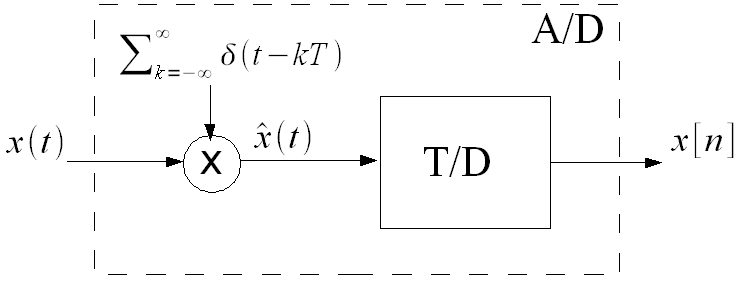
\includegraphics[width=7.5cm]{AD.png}
$\qquad$
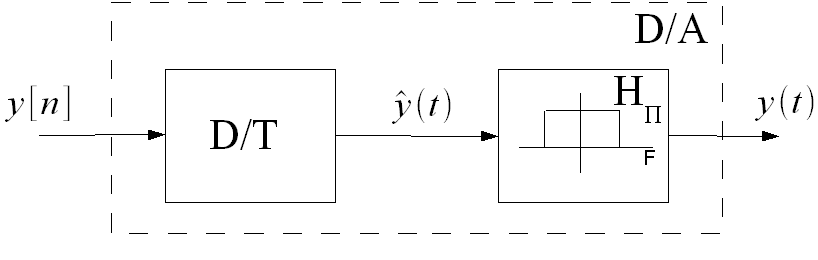
\includegraphics[width=7.5cm]{DA.png}
\end{center}
\end{figure}

El proc\'es de conversi\'o d'anal\`ogic a digital es pot descriure, de manera ideal, en dues etapes: el producte
del senyal anal\`ogic per un tren de deltes i la conversi\'o del resultat (bloc \textbf{T/D}) en la seva versi\'o 
discreta. Processos com la quantificaci\'o i codificaci\'o dels valors del senyal no es tenen en compte.
La relació entre els senyals $x(t)$, $\hat{x}(t)$ i $x[n]$ és l'explicada en la secció \textit{Mostreig de senyals}.

\vskip 0.3 cm
El proc\'es de conversi\'o de digital a anal\`ogic es pot descriure, de manera ideal, en dues etapes:
el pas a la versi\'o cont\'inua del senyal discret, expressat com a tren de deltes (bloc \textbf{D/T})
i eliminaci\'o de les repeticions de la transformada (bloc \textit{filtre passa-baix}, amb funci\'o de
transfer\`encia $H_{\Pi}(F)$\footnote{$H_{\Pi}(F)=\begin{cases} T & \text{ si } |F| \leq 1/2T \\ 0 & \text{altrament} \end{cases}$,
o en termes de $\Omega$: $H_{\Omega}(F)=\begin{cases} T & \text{ si } |\Omega| \leq \pi/T \\ 0 & \text{altrament} \end{cases}$}). 
La relació entre els senyals $y[n]$, $\hat{y}(t)$ i $y(t)$ és l'explicada en la secció \textit{Mostreig de senyals}.

\vskip 0.3 cm
\noindent
La seg\"uent figura mostra dos exemples de conversi\'o D/A i A/D:

\begin{figure}[htbp]
\begin{center}
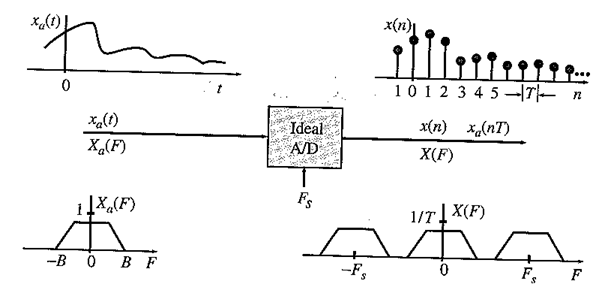
\includegraphics[width=7cm]{exAD.png}
$\qquad$ $\quad$
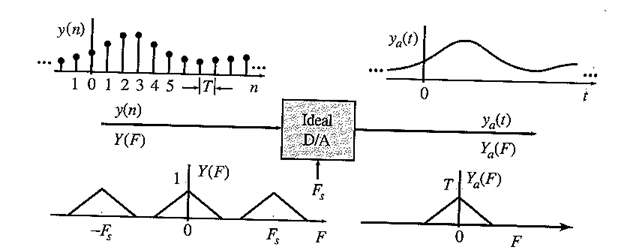
\includegraphics[width=7.5cm]{exDA.png}
\end{center}
\end{figure}


La transformada de Fourier del senyal de sortida $Y_a(F)$ es pot escriure en funci\'o de tots els blocs
del sistema de la seg\"uent manera:

\[
Y_a(F)=H_{\Pi}(f) \cdot H(FT) \cdot \frac{1}{T} \sum_{k=-\infty}^\infty X_a(F-\frac{k}{T})=H(FT) \cdot X_a(F)
\]


\vskip 2cm
\noindent
\textbf{Nota:} la majoria de figures d'aquest cap\'itol s'han tret de Digital Signal Processing, J. Proakis, D. Manolakis, Pearson Prentice Hall, 2007.



\end{document}
